% Generated by Sphinx.
\def\sphinxdocclass{report}
\documentclass[letterpaper,10pt,english]{sphinxmanual}
\usepackage[utf8]{inputenc}
\DeclareUnicodeCharacter{00A0}{\nobreakspace}
\usepackage{cmap}
\usepackage[T1]{fontenc}
\usepackage{babel}
\usepackage{times}
\usepackage[Bjarne]{fncychap}
\usepackage{longtable}
\usepackage{sphinx}
\usepackage{multirow}

\addto\captionsenglish{\renewcommand{\figurename}{Fig. }}
\addto\captionsenglish{\renewcommand{\tablename}{Table }}
\floatname{literal-block}{Listing }

\usepackage{amsfonts,amsmath}

\title{CySparse's users manual}
\date{December 23, 2015}
\release{0.2.2}
\author{Nikolaj van Omme\\Sylvain Arreckx\\Dominique Orban}
\newcommand{\sphinxlogo}{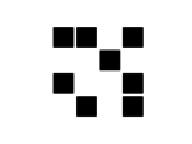
\includegraphics{cysparse_logo128.pdf}\par}
\renewcommand{\releasename}{Release}
\makeindex

\makeatletter
\def\PYG@reset{\let\PYG@it=\relax \let\PYG@bf=\relax%
    \let\PYG@ul=\relax \let\PYG@tc=\relax%
    \let\PYG@bc=\relax \let\PYG@ff=\relax}
\def\PYG@tok#1{\csname PYG@tok@#1\endcsname}
\def\PYG@toks#1+{\ifx\relax#1\empty\else%
    \PYG@tok{#1}\expandafter\PYG@toks\fi}
\def\PYG@do#1{\PYG@bc{\PYG@tc{\PYG@ul{%
    \PYG@it{\PYG@bf{\PYG@ff{#1}}}}}}}
\def\PYG#1#2{\PYG@reset\PYG@toks#1+\relax+\PYG@do{#2}}

\expandafter\def\csname PYG@tok@gd\endcsname{\def\PYG@tc##1{\textcolor[rgb]{0.63,0.00,0.00}{##1}}}
\expandafter\def\csname PYG@tok@gu\endcsname{\let\PYG@bf=\textbf\def\PYG@tc##1{\textcolor[rgb]{0.50,0.00,0.50}{##1}}}
\expandafter\def\csname PYG@tok@gt\endcsname{\def\PYG@tc##1{\textcolor[rgb]{0.00,0.27,0.87}{##1}}}
\expandafter\def\csname PYG@tok@gs\endcsname{\let\PYG@bf=\textbf}
\expandafter\def\csname PYG@tok@gr\endcsname{\def\PYG@tc##1{\textcolor[rgb]{1.00,0.00,0.00}{##1}}}
\expandafter\def\csname PYG@tok@cm\endcsname{\let\PYG@it=\textit\def\PYG@tc##1{\textcolor[rgb]{0.25,0.50,0.56}{##1}}}
\expandafter\def\csname PYG@tok@vg\endcsname{\def\PYG@tc##1{\textcolor[rgb]{0.73,0.38,0.84}{##1}}}
\expandafter\def\csname PYG@tok@m\endcsname{\def\PYG@tc##1{\textcolor[rgb]{0.13,0.50,0.31}{##1}}}
\expandafter\def\csname PYG@tok@mh\endcsname{\def\PYG@tc##1{\textcolor[rgb]{0.13,0.50,0.31}{##1}}}
\expandafter\def\csname PYG@tok@cs\endcsname{\def\PYG@tc##1{\textcolor[rgb]{0.25,0.50,0.56}{##1}}\def\PYG@bc##1{\setlength{\fboxsep}{0pt}\colorbox[rgb]{1.00,0.94,0.94}{\strut ##1}}}
\expandafter\def\csname PYG@tok@ge\endcsname{\let\PYG@it=\textit}
\expandafter\def\csname PYG@tok@vc\endcsname{\def\PYG@tc##1{\textcolor[rgb]{0.73,0.38,0.84}{##1}}}
\expandafter\def\csname PYG@tok@il\endcsname{\def\PYG@tc##1{\textcolor[rgb]{0.13,0.50,0.31}{##1}}}
\expandafter\def\csname PYG@tok@go\endcsname{\def\PYG@tc##1{\textcolor[rgb]{0.20,0.20,0.20}{##1}}}
\expandafter\def\csname PYG@tok@cp\endcsname{\def\PYG@tc##1{\textcolor[rgb]{0.00,0.44,0.13}{##1}}}
\expandafter\def\csname PYG@tok@gi\endcsname{\def\PYG@tc##1{\textcolor[rgb]{0.00,0.63,0.00}{##1}}}
\expandafter\def\csname PYG@tok@gh\endcsname{\let\PYG@bf=\textbf\def\PYG@tc##1{\textcolor[rgb]{0.00,0.00,0.50}{##1}}}
\expandafter\def\csname PYG@tok@ni\endcsname{\let\PYG@bf=\textbf\def\PYG@tc##1{\textcolor[rgb]{0.84,0.33,0.22}{##1}}}
\expandafter\def\csname PYG@tok@nl\endcsname{\let\PYG@bf=\textbf\def\PYG@tc##1{\textcolor[rgb]{0.00,0.13,0.44}{##1}}}
\expandafter\def\csname PYG@tok@nn\endcsname{\let\PYG@bf=\textbf\def\PYG@tc##1{\textcolor[rgb]{0.05,0.52,0.71}{##1}}}
\expandafter\def\csname PYG@tok@no\endcsname{\def\PYG@tc##1{\textcolor[rgb]{0.38,0.68,0.84}{##1}}}
\expandafter\def\csname PYG@tok@na\endcsname{\def\PYG@tc##1{\textcolor[rgb]{0.25,0.44,0.63}{##1}}}
\expandafter\def\csname PYG@tok@nb\endcsname{\def\PYG@tc##1{\textcolor[rgb]{0.00,0.44,0.13}{##1}}}
\expandafter\def\csname PYG@tok@nc\endcsname{\let\PYG@bf=\textbf\def\PYG@tc##1{\textcolor[rgb]{0.05,0.52,0.71}{##1}}}
\expandafter\def\csname PYG@tok@nd\endcsname{\let\PYG@bf=\textbf\def\PYG@tc##1{\textcolor[rgb]{0.33,0.33,0.33}{##1}}}
\expandafter\def\csname PYG@tok@ne\endcsname{\def\PYG@tc##1{\textcolor[rgb]{0.00,0.44,0.13}{##1}}}
\expandafter\def\csname PYG@tok@nf\endcsname{\def\PYG@tc##1{\textcolor[rgb]{0.02,0.16,0.49}{##1}}}
\expandafter\def\csname PYG@tok@si\endcsname{\let\PYG@it=\textit\def\PYG@tc##1{\textcolor[rgb]{0.44,0.63,0.82}{##1}}}
\expandafter\def\csname PYG@tok@s2\endcsname{\def\PYG@tc##1{\textcolor[rgb]{0.25,0.44,0.63}{##1}}}
\expandafter\def\csname PYG@tok@vi\endcsname{\def\PYG@tc##1{\textcolor[rgb]{0.73,0.38,0.84}{##1}}}
\expandafter\def\csname PYG@tok@nt\endcsname{\let\PYG@bf=\textbf\def\PYG@tc##1{\textcolor[rgb]{0.02,0.16,0.45}{##1}}}
\expandafter\def\csname PYG@tok@nv\endcsname{\def\PYG@tc##1{\textcolor[rgb]{0.73,0.38,0.84}{##1}}}
\expandafter\def\csname PYG@tok@s1\endcsname{\def\PYG@tc##1{\textcolor[rgb]{0.25,0.44,0.63}{##1}}}
\expandafter\def\csname PYG@tok@gp\endcsname{\let\PYG@bf=\textbf\def\PYG@tc##1{\textcolor[rgb]{0.78,0.36,0.04}{##1}}}
\expandafter\def\csname PYG@tok@sh\endcsname{\def\PYG@tc##1{\textcolor[rgb]{0.25,0.44,0.63}{##1}}}
\expandafter\def\csname PYG@tok@ow\endcsname{\let\PYG@bf=\textbf\def\PYG@tc##1{\textcolor[rgb]{0.00,0.44,0.13}{##1}}}
\expandafter\def\csname PYG@tok@sx\endcsname{\def\PYG@tc##1{\textcolor[rgb]{0.78,0.36,0.04}{##1}}}
\expandafter\def\csname PYG@tok@bp\endcsname{\def\PYG@tc##1{\textcolor[rgb]{0.00,0.44,0.13}{##1}}}
\expandafter\def\csname PYG@tok@c1\endcsname{\let\PYG@it=\textit\def\PYG@tc##1{\textcolor[rgb]{0.25,0.50,0.56}{##1}}}
\expandafter\def\csname PYG@tok@kc\endcsname{\let\PYG@bf=\textbf\def\PYG@tc##1{\textcolor[rgb]{0.00,0.44,0.13}{##1}}}
\expandafter\def\csname PYG@tok@c\endcsname{\let\PYG@it=\textit\def\PYG@tc##1{\textcolor[rgb]{0.25,0.50,0.56}{##1}}}
\expandafter\def\csname PYG@tok@mf\endcsname{\def\PYG@tc##1{\textcolor[rgb]{0.13,0.50,0.31}{##1}}}
\expandafter\def\csname PYG@tok@err\endcsname{\def\PYG@bc##1{\setlength{\fboxsep}{0pt}\fcolorbox[rgb]{1.00,0.00,0.00}{1,1,1}{\strut ##1}}}
\expandafter\def\csname PYG@tok@mb\endcsname{\def\PYG@tc##1{\textcolor[rgb]{0.13,0.50,0.31}{##1}}}
\expandafter\def\csname PYG@tok@ss\endcsname{\def\PYG@tc##1{\textcolor[rgb]{0.32,0.47,0.09}{##1}}}
\expandafter\def\csname PYG@tok@sr\endcsname{\def\PYG@tc##1{\textcolor[rgb]{0.14,0.33,0.53}{##1}}}
\expandafter\def\csname PYG@tok@mo\endcsname{\def\PYG@tc##1{\textcolor[rgb]{0.13,0.50,0.31}{##1}}}
\expandafter\def\csname PYG@tok@kd\endcsname{\let\PYG@bf=\textbf\def\PYG@tc##1{\textcolor[rgb]{0.00,0.44,0.13}{##1}}}
\expandafter\def\csname PYG@tok@mi\endcsname{\def\PYG@tc##1{\textcolor[rgb]{0.13,0.50,0.31}{##1}}}
\expandafter\def\csname PYG@tok@kn\endcsname{\let\PYG@bf=\textbf\def\PYG@tc##1{\textcolor[rgb]{0.00,0.44,0.13}{##1}}}
\expandafter\def\csname PYG@tok@o\endcsname{\def\PYG@tc##1{\textcolor[rgb]{0.40,0.40,0.40}{##1}}}
\expandafter\def\csname PYG@tok@kr\endcsname{\let\PYG@bf=\textbf\def\PYG@tc##1{\textcolor[rgb]{0.00,0.44,0.13}{##1}}}
\expandafter\def\csname PYG@tok@s\endcsname{\def\PYG@tc##1{\textcolor[rgb]{0.25,0.44,0.63}{##1}}}
\expandafter\def\csname PYG@tok@kp\endcsname{\def\PYG@tc##1{\textcolor[rgb]{0.00,0.44,0.13}{##1}}}
\expandafter\def\csname PYG@tok@w\endcsname{\def\PYG@tc##1{\textcolor[rgb]{0.73,0.73,0.73}{##1}}}
\expandafter\def\csname PYG@tok@kt\endcsname{\def\PYG@tc##1{\textcolor[rgb]{0.56,0.13,0.00}{##1}}}
\expandafter\def\csname PYG@tok@sc\endcsname{\def\PYG@tc##1{\textcolor[rgb]{0.25,0.44,0.63}{##1}}}
\expandafter\def\csname PYG@tok@sb\endcsname{\def\PYG@tc##1{\textcolor[rgb]{0.25,0.44,0.63}{##1}}}
\expandafter\def\csname PYG@tok@k\endcsname{\let\PYG@bf=\textbf\def\PYG@tc##1{\textcolor[rgb]{0.00,0.44,0.13}{##1}}}
\expandafter\def\csname PYG@tok@se\endcsname{\let\PYG@bf=\textbf\def\PYG@tc##1{\textcolor[rgb]{0.25,0.44,0.63}{##1}}}
\expandafter\def\csname PYG@tok@sd\endcsname{\let\PYG@it=\textit\def\PYG@tc##1{\textcolor[rgb]{0.25,0.44,0.63}{##1}}}

\def\PYGZbs{\char`\\}
\def\PYGZus{\char`\_}
\def\PYGZob{\char`\{}
\def\PYGZcb{\char`\}}
\def\PYGZca{\char`\^}
\def\PYGZam{\char`\&}
\def\PYGZlt{\char`\<}
\def\PYGZgt{\char`\>}
\def\PYGZsh{\char`\#}
\def\PYGZpc{\char`\%}
\def\PYGZdl{\char`\$}
\def\PYGZhy{\char`\-}
\def\PYGZsq{\char`\'}
\def\PYGZdq{\char`\"}
\def\PYGZti{\char`\~}
% for compatibility with earlier versions
\def\PYGZat{@}
\def\PYGZlb{[}
\def\PYGZrb{]}
\makeatother

\renewcommand\PYGZsq{\textquotesingle}

\begin{document}

\maketitle
\tableofcontents
\phantomsection\label{contents::doc}

\begin{quote}\begin{description}
\item[{Release}] \leavevmode
0.2

\item[{Date}] \leavevmode
December 23, 2015

\end{description}\end{quote}


\chapter{Introduction}
\label{introduction:introduction}\label{introduction:cysparse-s-users-manual}\label{introduction::doc}
Welcome to \textbf{\texttt{CySparse}}`s users manual!

We tried to keep this manual as simple and short as possible. You can find much more detailed information in the developer's manual.
To see \textbf{\texttt{CySparse}} in action, you can try the tutorials written in \href{http://ipython.org/notebook.html}{IPython Notebooks} or run the examples in the
\code{examples} directory.


\section{What is \textbf{\texttt{CySparse}}?}
\label{introduction:what-is-cysparse}
\textbf{\texttt{CySparse}} is a fast sparse matrix library for \textbf{\texttt{Python}}/\textbf{\texttt{Cython}}.


\section{Content}
\label{introduction:content}

\section{\textbf{\texttt{PySparse}} legacy}
\label{introduction:pysparse-legacy}

\section{\textbf{\texttt{PySparse}} vs \textbf{\texttt{CySparse}}}
\label{introduction:pysparse-vs-cysparse}
Even if \textbf{\texttt{CySparse}} is (strongly) inspired from \textbf{\texttt{PySparse}}, there are notable differences. In short, \textbf{\texttt{CySparse}}:
\begin{itemize}
\item {} 
allows the use of matrices with \textbf{different types} of indices and elements at run time (see ...);

\item {} 
is \textbf{faster} than \textbf{\texttt{PySparse}} (see ...);

\item {} 
uses \textbf{matrix views} - a very light proxy object - that represent parts of a matrix without the need to copy elements (see...);

\item {} 
has more \textbf{syntaxic sugar}, like \code{A * b, b * A, A.T * b} etc.

\item {} 
has a \textbf{symmetric} version of \textbf{all} its matrix types.

\item {} 
\textbf{doesn't use masks}.

\end{itemize}

Both libraries define similar but also different matrix classes:
\begin{quote}

\begin{tabular}{|p{0.317\linewidth}|p{0.317\linewidth}|p{0.317\linewidth}|}
\hline
\textsf{\relax 
Matrix type
} & \textsf{\relax 
\textbf{\texttt{PySparse}}
} & \textsf{\relax 
\textbf{\texttt{CySparse}}
}\\
\hline
Linked-List Format
 & 
\code{ll\_mat}, \code{ll\_mat\_sym}, \code{PysparseMatrix}
 & 
\code{LLSparseMatrix}
\\
\hline
Compressed Sparse Row Format
 & 
\code{csr\_mat}
 & 
\code{CSRSparseMatrix}
\\
\hline
Compressed Sparse Column Format
 & \begin{itemize}
\item {} 
\end{itemize}
 & 
\code{CSCSparseMatrix}
\\
\hline
Sparse Skyline Format
 & 
\code{sss\_mat}
 & \begin{itemize}
\item {} 
\end{itemize}
\\
\hline
Compressed Sparse Row and Column Format
 & \begin{itemize}
\item {} 
\end{itemize}
 & 
\code{CSBSparseMatrix}
\\
\hline\end{tabular}

\end{quote}


\section{License}
\label{introduction:license}

\chapter{\textbf{\texttt{CySparse}} installation}
\label{installation:cysparse-installation}\label{installation::doc}
There are basically \footnote{
Some special configurations might need a complete or partial \textbf{\texttt{Cython}} source generation.
}, two modes to install \textbf{\texttt{CySparse}}:
\begin{itemize}
\item {} 
\textbf{\texttt{Python}} mode and

\item {} 
\textbf{\texttt{Cython}} mode.

\end{itemize}

In \textbf{\texttt{Python}} mode, you install the library as a usual \textbf{\texttt{Python}} library. In \textbf{\texttt{Cython}} mode a little bit more work is involved as you also need to generate the source code from templated files.

The installation is done in a few simple steps:
\begin{enumerate}
\item {} 
Clone the repository;

\item {} 
Install the dependencies;

\item {} 
Tweak the configuration file \code{cysparse.cfg};

\item {} 
Generate the source code if needed (i.e. in \textbf{\texttt{Cython}} mode);

\item {} 
Compile and install the library:

\end{enumerate}

We detail these steps in the next sections for both installation modes.


\section{\textbf{\texttt{Python}} installation mode}
\label{installation:python-installation-mode}

\subsection{Clone the repository}
\label{installation:clone-the-repository}

\subsection{Install the depencies}
\label{installation:install-the-depencies}
All \textbf{\texttt{Python}} dependencies are described in the \code{requirements.txt} files. You can easily install them all with:

\begin{Verbatim}[commandchars=\\\{\}]
pip install \PYGZhy{}r requirements.txt
\end{Verbatim}

or a similar command. Other dependencies need some manual installation. Read further.


\subsubsection{\textbf{\texttt{CySparse}}}
\label{installation:cysparse}\begin{itemize}
\item {} 
\textbf{\texttt{Cython}}

\item {} 
\textbf{\texttt{Jinja2}}

\item {} 
argparse

\item {} 
fortranformat

\item {} 
\textbf{\texttt{SuiteSparse}} (for the moment, it not possible to install \textbf{\texttt{CySparse}} \textbf{without} \textbf{\texttt{SuiteSparse}})

\end{itemize}


\subsubsection{Documentation}
\label{installation:documentation}\begin{itemize}
\item {} 
\textbf{\texttt{Sphinx}}

\item {} 
sphinx-bootstrap-theme

\end{itemize}


\subsubsection{Unit testing}
\label{installation:unit-testing}\begin{itemize}
\item {} 
\textbf{\texttt{PySparse}}

\end{itemize}


\subsubsection{Performance testing}
\label{installation:performance-testing}\begin{itemize}
\item {} 
\textbf{\texttt{PySparse}}

\item {} 
benchmark.py (\href{https://github.com/optimizers/benchmark.py}{https://github.com/optimizers/benchmark.py})

\end{itemize}


\subsection{Tweak the configuration file \texttt{cysparse.cfg}}
\label{installation:tweak-the-configuration-file-cysparse-cfg}
{[}THIS IS WORK IN PROGRESS{]}

\# log file name \textbf{without} extension (by default, we use `.log')
log\_name = cysparse\_generate\_code
\# DEBUG/INFO/WARNING/ERROR/CRITICAL
log\_level = INFO
console\_log\_level = WARNING
file\_log\_level = WARNING

\# 32bits/64bits
\# if left blank, we use INT64\_t on 64 bits platforms and INT32\_t on 32 bits platforms
DEFAULT\_INDEX\_TYPE =


\subsection{Generate the source code}
\label{installation:generate-the-source-code}
Some parts of the library source code have to be generated \textbf{if} you use \textbf{\texttt{Cython}} or wish to generate the code from scratch. We use a script:

\begin{Verbatim}[commandchars=\\\{\}]
python generate\PYGZus{}code.py \PYGZhy{}a
\end{Verbatim}

The switch \code{-a} stands for \code{-{-}all} and generates the entire library. If you need help, try the \code{-h} switch.


\subsection{Compile and install the library}
\label{installation:compile-and-install-the-library}
The preferred way to install the library is to install it in its own \emph{virtualenv}.

Wheter using a virtual environment or not, use the traditionnal:

\begin{Verbatim}[commandchars=\\\{\}]
python setup.py install
\end{Verbatim}

to compile and install the library.


\section{\textbf{\texttt{Cython}} installation mode}
\label{installation:cython-installation-mode}

\subsection{Inconveniences}
\label{installation:inconveniences}\begin{itemize}
\item {} 
Sometimes \textbf{\texttt{Cython}} can ask for a complete recompilation.
Whenever this happens, it displays the following message when trying to import the library
into \textbf{\texttt{Python}}:

\begin{Verbatim}[commandchars=\\\{\}]
ValueError: XXX has the wrong size, try recompiling
\end{Verbatim}

where XXX is the first class that has the wrong size. The easiest way to deal with this is to recompile all the .pyx files again (you can force this by removing
all the .c files) \footnote{
The problem is interdependencies between source files that are not catched at compile time. Whenever \textbf{\texttt{Cython}} can catch them at runtime, it throws this \code{ValueError}.
}.

See Robert Bradshaw's \href{https://groups.google.com/forum/?hl=en\#!topic/cython-users/cOAVM0whJkY}{answer}.
See also \href{https://github.com/cython/cython/wiki/enhancements-distutils\_preprocessing}{enhancements distutils\_preprocessing}.

\item {} 
\textbf{If} you modify the templated code, some dependencies might be missing in the (generated) \code{setup.py} file and require manual intervention,
i.e. recompilation. The easiest way to go is to recompile everything from scratch \footnote{
Interdependencies between generated templates are \textbf{not} monitored. Instead of recompiling everything from scratch, you can also simply delete the corresponding \textbf{\texttt{Cython}} generated files. This will spare you some compilation time.
}. First delete the generated files:

\begin{Verbatim}[commandchars=\\\{\}]
python generate\PYGZus{}code.py \PYGZhy{}ac
\end{Verbatim}

where \code{-ac} stands for \code{a}ll and \code{c}lean. This will delete \textbf{all} generated \code{.pxi}, \code{.pxd} and \code{.pyx} \textbf{\texttt{Cython}} files. Then delete the generated \textbf{\texttt{C}} files:

\begin{Verbatim}[commandchars=\\\{\}]
python clean.py
\end{Verbatim}

This will delete \textbf{all} \textbf{\texttt{C}} \code{.c} files. You can then recompile the library from scratch.

\end{itemize}


\chapter{\textbf{\texttt{CySparse}}`s types}
\label{types:cysparse-s-types}\label{types:cysparse-types}\label{types::doc}
Internally, \textbf{\texttt{CySparse}} uses typed variables. As a \textbf{\texttt{Python}} user, you don't have directly access to these types but you can ask for a specific type to be used through the use of simple (enum) arguments.
As a \textbf{\texttt{Cython}} user however, you do have access to these types and you can (and should) use them in your \textbf{\texttt{Cython}} programs. For every type, there is a corresponding (enum) argument. Types are written with
\code{\_t} as suffix: \code{INT32\_t}, \code{COMPLEX256\_t}. The corresponding (enum) arguments are simply the names of the types with \code{\_T} as suffix. Thus the (enum) argument corresponding to type \code{FLOAT64\_t} is \code{FLOAT64\_T}
(notice the capital \code{T}).


\section{Compatibility with \textbf{\texttt{NumPy}}}
\label{types:compatibility-with-numpy}
In short, \textbf{\texttt{CySparse}}`s types  are 100\% compatible with the \textbf{\texttt{NumPy}} corresponding types \footnote{
Behind the hood, both libraries use \textbf{\texttt{C99}} types (whenever \textbf{\texttt{NumPy}} is compiled with a \textbf{\texttt{C99}} compliant compiler).
\textbf{\texttt{CySparse}} doesn't offer as many different types as \textbf{\texttt{NumPy}} though«.
}.
There are some differences thought between the way both libraries treat their types and numbers. Read on.

\begin{notice}{warning}{Warning:}
The behavior of similar types in \textbf{\texttt{NumPy}} and \textbf{\texttt{CySparse}} can be different!
\end{notice}


\section{Available types}
\label{types:availabe-types}\label{types:available-types}
\textbf{\texttt{CySparse}} has some types that can be used for indices and some types that can be used for elements.


\subsection{Indices: integer numbers}
\label{types:indices-integer-numbers}
Two index types exist: signed 32 and signed 64 bits integers. Internally, they are named \code{INT32\_t} and \code{ÌNT64\_t}.


\subsection{Elements: integers, real and complex numbers}
\label{types:elements-integers-real-and-complex-numbers}
\textbf{\texttt{CySparse}} has three different families of element types:
\begin{itemize}
\item {} 
integers: simple and double precision signed integers (\code{INT32\_t} and \code{INT64\_t}).

\item {} 
real numbers: simple, double and quadruple precision real numbers (\code{FLOAT32\_t}, \code{FLOAT64\_t} and \code{FLOAT128\_t}).

\item {} 
complex numbers: simple and double precision complex numbers (\code{COMPLEX64\_t}, \code{COMPLEX128\_t}, \code{COMPLEX256\_t}).

\end{itemize}

Quadruple precision has some limited support in \textbf{\texttt{C99}} standard and \textbf{\texttt{Cython}} and thus in \textbf{\texttt{CySparse}}. The same can be said about complex number in general although the simple and double precision are quite
well integrated. This is worth a warning:

\begin{notice}{warning}{Warning:}
Quadruple precision and complex numbers have some limitations.
\end{notice}


\section{Number's behavior in \textbf{\texttt{CySparse}}}
\label{types:number-s-behavior-in-cysparse}
The three families of element types behave somewhat differently.


\subsection{Overflow on assignment}
\label{types:overflow-on-assignment}
Numbers do overflow \footnote{
Overflow is compiler-dependent (and compilers are often system-dependent).
}. When assigning an integer number a value too big for its type, an \code{OverflowError} is raised.

\begin{Verbatim}[commandchars=\\\{\}]
\PYG{n}{B} \PYG{o}{=} \PYG{n}{ll\PYGZus{}mat}\PYG{o}{.}\PYG{n}{NewLLSparseMatrix}\PYG{p}{(}\PYG{n}{size}\PYG{o}{=}\PYG{l+m+mi}{2}\PYG{p}{,} \PYG{n}{dtype}\PYG{o}{=}\PYG{n}{types}\PYG{o}{.}\PYG{n}{INT32\PYGZus{}T}\PYG{p}{)}

\PYG{n}{B}\PYG{p}{[}\PYG{l+m+mi}{1}\PYG{p}{,} \PYG{l+m+mi}{1}\PYG{p}{]} \PYG{o}{=} \PYG{l+m+mi}{2}\PYG{o}{*}\PYG{o}{*}\PYG{l+m+mi}{31}
\end{Verbatim}

raises an \code{OverflowError} with the following message:

\begin{Verbatim}[commandchars=\\\{\}]
Traceback \PYG{o}{(}most recent call last\PYG{o}{)}:
  File \PYG{l+s+s2}{\PYGZdq{}new\PYGZus{}types.py\PYGZdq{}}, line 102, in \PYGZlt{}module\PYGZgt{}
    B\PYG{o}{[}1, 1\PYG{o}{]} \PYG{o}{=} 2**31
  File \PYG{l+s+s2}{\PYGZdq{}cysparse/sparse/ll\PYGZus{}mat\PYGZus{}matrices/ll\PYGZus{}mat\PYGZus{}INT32\PYGZus{}t\PYGZus{}INT32\PYGZus{}t.pyx\PYGZdq{}}, line 538, in cysparse.sparse.ll\PYGZus{}mat\PYGZus{}matrices.ll\PYGZus{}mat\PYGZus{}INT32\PYGZus{}t\PYGZus{}INT32\PYGZus{}t.LLSparseMatrix\PYGZus{}INT32\PYGZus{}t\PYGZus{}INT32\PYGZus{}t.\PYGZus{}\PYGZus{}setitem\PYGZus{}\PYGZus{} \PYG{o}{(}cysparse/sparse/ll\PYGZus{}mat\PYGZus{}matrices/ll\PYGZus{}mat\PYGZus{}INT32\PYGZus{}t\PYGZus{}INT32\PYGZus{}t.c:6565\PYG{o}{)}
OverflowError: value too large to convert to int
\end{Verbatim}

When assigning a real or complex number a value that is too big for its type,
it is assigned \emph{inf}, i.e. \(+\infty\) \textbf{without} any warning:

\begin{Verbatim}[commandchars=\\\{\}]
\PYG{n}{B} \PYG{o}{=} \PYG{n}{ll\PYGZus{}mat}\PYG{o}{.}\PYG{n}{NewLLSparseMatrix}\PYG{p}{(}\PYG{n}{size}\PYG{o}{=}\PYG{l+m+mi}{2}\PYG{p}{,} \PYG{n}{dtype}\PYG{o}{=}\PYG{n}{types}\PYG{o}{.}\PYG{n}{FLOAT32\PYGZus{}T}\PYG{p}{)}

\PYG{n}{B}\PYG{p}{[}\PYG{l+m+mi}{0}\PYG{p}{,} \PYG{l+m+mi}{0}\PYG{p}{]} \PYG{o}{=} \PYG{l+m+mi}{232}
\PYG{n}{B}\PYG{p}{[}\PYG{l+m+mi}{0}\PYG{p}{,} \PYG{l+m+mi}{1}\PYG{p}{]} \PYG{o}{=} \PYG{l+m+mf}{1.3}
\PYG{n}{B}\PYG{p}{[}\PYG{l+m+mi}{1}\PYG{p}{,} \PYG{l+m+mi}{1}\PYG{p}{]} \PYG{o}{=} \PYG{l+m+mi}{2}\PYG{o}{*}\PYG{o}{*}\PYG{l+m+mi}{310}

\PYG{n}{B}\PYG{o}{.}\PYG{n}{print\PYGZus{}to}\PYG{p}{(}\PYG{n}{sys}\PYG{o}{.}\PYG{n}{stdout}\PYG{p}{)}
\end{Verbatim}

prints:

\begin{Verbatim}[commandchars=\\\{\}]
LLSparseMatrix \PYG{o}{[}INT32\PYGZus{}t, FLOAT32\PYGZus{}t\PYG{o}{]} \PYG{o}{(}G, NZ, \PYG{o}{[}2, 2\PYG{o}{]}\PYG{o}{)}
232.000000  1.300000
  0.000000       inf
\end{Verbatim}


\subsection{Overflow on operation}
\label{types:overflow-on-operation}
We follow the \textbf{\texttt{C99}} standard and let an overflow during an operation pass silently (and give strange results) without a warning.

Let's define a matrix with huge numbers:

\begin{Verbatim}[commandchars=\\\{\}]
\PYG{n}{B} \PYG{o}{=} \PYG{n}{ll\PYGZus{}mat}\PYG{o}{.}\PYG{n}{NewLLSparseMatrix}\PYG{p}{(}\PYG{n}{size}\PYG{o}{=}\PYG{l+m+mi}{2}\PYG{p}{,} \PYG{n}{dtype}\PYG{o}{=}\PYG{n}{types}\PYG{o}{.}\PYG{n}{INT32\PYGZus{}T}\PYG{p}{)}

\PYG{n}{B}\PYG{p}{[}\PYG{l+m+mi}{0}\PYG{p}{,} \PYG{l+m+mi}{0}\PYG{p}{]} \PYG{o}{=} \PYG{l+m+mi}{232}
\PYG{n}{B}\PYG{p}{[}\PYG{l+m+mi}{0}\PYG{p}{,} \PYG{l+m+mi}{1}\PYG{p}{]} \PYG{o}{=} \PYG{l+m+mf}{1.3}
\PYG{n}{B}\PYG{p}{[}\PYG{l+m+mi}{1}\PYG{p}{,} \PYG{l+m+mi}{1}\PYG{p}{]} \PYG{o}{=} \PYG{l+m+mi}{2}\PYG{o}{*}\PYG{o}{*}\PYG{l+m+mi}{31} \PYG{o}{\PYGZhy{}}\PYG{l+m+mi}{1}

\PYG{n}{B}\PYG{o}{.}\PYG{n}{print\PYGZus{}to}\PYG{p}{(}\PYG{n}{sys}\PYG{o}{.}\PYG{n}{stdout}\PYG{p}{)}
\end{Verbatim}

This prints:

\begin{Verbatim}[commandchars=\\\{\}]
LLSparseMatrix \PYG{o}{[}INT32\PYGZus{}t, INT32\PYGZus{}t\PYG{o}{]} \PYG{o}{(}G, NZ, \PYG{o}{[}2, 2\PYG{o}{]}\PYG{o}{)}
\PYG{l+m}{232}          1
  \PYG{l+m}{0} 2147483647
\end{Verbatim}

Multiplying \code{B} by itself returns a strange result:

\begin{Verbatim}[commandchars=\\\{\}]
\PYG{n}{C} \PYG{o}{=} \PYG{n}{B} \PYG{o}{*} \PYG{n}{B}
\PYG{n}{C}\PYG{o}{.}\PYG{n}{print\PYGZus{}to}\PYG{p}{(}\PYG{n}{sys}\PYG{o}{.}\PYG{n}{stdout}\PYG{p}{)}
\end{Verbatim}

prints:

\begin{Verbatim}[commandchars=\\\{\}]
\PYG{l+m}{53824} \PYGZhy{}2147483417
    \PYG{l+m}{0}           1
\end{Verbatim}


\subsection{\texttt{nan} and \texttt{inf}}
\label{types:nan-and-inf}
Like \textbf{\texttt{NumPy}}, \textbf{\texttt{CySparse}} defines \code{nan} and \code{inf}. These are compatible with their \textbf{\texttt{NumPy}} counterparts and can be used interchangebly. They are used internally as the \emph{C99} standard recommends.

\begin{Verbatim}[commandchars=\\\{\}]
\PYG{k+kn}{import} \PYG{n+nn}{cysparse.types.cysparse\PYGZus{}types} \PYG{k+kn}{as} \PYG{n+nn}{types}

\PYG{n}{B} \PYG{o}{=} \PYG{n}{ll\PYGZus{}mat}\PYG{o}{.}\PYG{n}{NewLLSparseMatrix}\PYG{p}{(}\PYG{n}{size}\PYG{o}{=}\PYG{l+m+mi}{2}\PYG{p}{,} \PYG{n}{dtype}\PYG{o}{=}\PYG{n}{types}\PYG{o}{.}\PYG{n}{FLOAT64\PYGZus{}T}\PYG{p}{)}

\PYG{n}{B}\PYG{p}{[}\PYG{l+m+mi}{0}\PYG{p}{,} \PYG{l+m+mi}{0}\PYG{p}{]} \PYG{o}{=} \PYG{l+m+mi}{232}
\PYG{n}{B}\PYG{p}{[}\PYG{l+m+mi}{0}\PYG{p}{,} \PYG{l+m+mi}{1}\PYG{p}{]} \PYG{o}{=} \PYG{l+m+mf}{1.3}
\PYG{n}{B}\PYG{p}{[}\PYG{l+m+mi}{1}\PYG{p}{,} \PYG{l+m+mi}{1}\PYG{p}{]} \PYG{o}{=} \PYG{n}{types}\PYG{o}{.}\PYG{n}{inf}

\PYG{n}{B}\PYG{o}{.}\PYG{n}{print\PYGZus{}to}\PYG{p}{(}\PYG{n}{sys}\PYG{o}{.}\PYG{n}{stdout}\PYG{p}{)}
\end{Verbatim}

This prints:

\begin{Verbatim}[commandchars=\\\{\}]
LLSparseMatrix \PYG{o}{[}INT32\PYGZus{}t, FLOAT64\PYGZus{}t\PYG{o}{]} \PYG{o}{(}G, NZ, \PYG{o}{[}2, 2\PYG{o}{]}\PYG{o}{)}
232.000000  1.300000
  0.000000       inf
\end{Verbatim}

If we multiply \code{B} by itself, we obtain:

\begin{Verbatim}[commandchars=\\\{\}]
LLSparseMatrix \PYG{o}{[}INT32\PYGZus{}t, FLOAT64\PYGZus{}t\PYG{o}{]} \PYG{o}{(}G, NZ, \PYG{o}{[}2, 2\PYG{o}{]}\PYG{o}{)}
53824.000000       inf
    0.000000       inf
\end{Verbatim}

as expected.


\subsection{Types compatibilities (implicit castings)}
\label{types:types-compatibilities-implicit-castings}
Whenever an integer is assigned a real number, \textbf{\texttt{CySparse}} assigns the integer part, i.e. takes its \code{floor()} part.

\begin{Verbatim}[commandchars=\\\{\}]
\PYG{n}{B} \PYG{o}{=} \PYG{n}{ll\PYGZus{}mat}\PYG{o}{.}\PYG{n}{NewLLSparseMatrix}\PYG{p}{(}\PYG{n}{size}\PYG{o}{=}\PYG{l+m+mi}{2}\PYG{p}{,} \PYG{n}{dtype}\PYG{o}{=}\PYG{n}{types}\PYG{o}{.}\PYG{n}{INT64\PYGZus{}T}\PYG{p}{)}

\PYG{n}{B}\PYG{p}{[}\PYG{l+m+mi}{0}\PYG{p}{,} \PYG{l+m+mi}{0}\PYG{p}{]} \PYG{o}{=} \PYG{l+m+mi}{232}
\PYG{n}{B}\PYG{p}{[}\PYG{l+m+mi}{0}\PYG{p}{,} \PYG{l+m+mi}{1}\PYG{p}{]} \PYG{o}{=} \PYG{l+m+mf}{1.3}
\PYG{n}{B}\PYG{p}{[}\PYG{l+m+mi}{1}\PYG{p}{,} \PYG{l+m+mi}{1}\PYG{p}{]} \PYG{o}{=} \PYG{o}{\PYGZhy{}}\PYG{l+m+mf}{0.89}
\end{Verbatim}

This matrix is in fact:

\begin{Verbatim}[commandchars=\\\{\}]
LLSparseMatrix \PYG{o}{[}INT32\PYGZus{}t, INT64\PYGZus{}t\PYG{o}{]} \PYG{o}{(}G, NZ, \PYG{o}{[}2, 2\PYG{o}{]}\PYG{o}{)}
\PYG{l+m}{232}  1
  \PYG{l+m}{0}  0
\end{Verbatim}

Complex number are compatible between them if they don't overflow but otherwise are \textbf{not} compatible
nor with the integer neither with the real numbers.

{[}TO BE DONE: write an example with complex numbers{]}


\chapter{\textbf{\texttt{CySparse}}`s basics}
\label{cysparse_basics:cysparse-s-basics}\label{cysparse_basics:cysparse-basics}\label{cysparse_basics::doc}
In this section, we explain the very basics of \textbf{\texttt{CySparse}}. Most matrices share some common basic attributes that we detail here.

Most attributes and \textbf{all} common ones are \emph{read-only}. Some attributes ask for some expensive computation. We indicate whenever this is the case.
Some attributes can also be given as arguments to most factory methods. We also detail which ones.


\section{Common strorage attributes}
\label{cysparse_basics:common-strorage-attributes}
For efficiency reasons, \textbf{\texttt{CySparse}} can use different storage schemes/methods to store matrices. For instance, symmetric matrices can be stored with only half of their elements.


\subsection{\texttt{store\_symmetric}}
\label{cysparse_basics:store-symmetric}
Symmetric matrices can be stored by only storing the \textbf{lower} triangular part and the diagonal of a matrix. To create a symmetric matrix, add the arguement \code{store\_symmetric=True} to the call of one of the factory methods.
The attribute \code{store\_symmetric} returns if this storage method is used or not. Thus, if \code{store\_symmetric} is \code{True}, you know that you deal with a symmetric matrix \textbf{and} that roughly only half of its elements are stored. If
\code{store\_symmetric} is \code{False}, it simply means that this storage scheme is not used. The matrix itself migth be symmetric or not.


\subsection{\texttt{store\_zero}}
\label{cysparse_basics:store-zero}
By default non specified (implicit) elements are zero (\code{0}, \code{0.0} or \code{0+0j}). \textbf{\texttt{CySparse}} allow the user to store explicitely zeros. To explicitely store zeros, declare \code{store\_zero=True} as an argument
in any factory method:

\begin{Verbatim}[commandchars=\\\{\}]
\PYG{n}{A} \PYG{o}{=} \PYG{n}{LLSparseMatrix}\PYG{p}{(}\PYG{n}{store\PYGZus{}zero}\PYG{o}{=}\PYG{n+nb+bp}{True}\PYG{p}{,} \PYG{o}{.}\PYG{o}{.}\PYG{o}{.}\PYG{p}{)}
\end{Verbatim}

The matrix \code{A} will store any zero explicitely as will any matrix created from it. You can access the value of this attribute:

\begin{Verbatim}[commandchars=\\\{\}]
\PYG{n}{A}\PYG{o}{.}\PYG{n}{store\PYGZus{}zero}
\end{Verbatim}

returns \code{True} for our example. This attribute is read-only and cannot be changed. If you want to temporarily exclude zeros in some operations, you can use the \code{NonZeros} context manager:

\begin{Verbatim}[commandchars=\\\{\}]
\PYG{k}{with} \PYG{n}{NonZeros}\PYG{p}{(}\PYG{n}{A}\PYG{p}{)}\PYG{p}{:}
    \PYG{c}{\PYGZsh{} use some method to add entries to A but disregard zeros entries}
    \PYG{o}{.}\PYG{o}{.}\PYG{o}{.}
\end{Verbatim}

This context manager temporarily set the \code{store\_zero} attribute to \code{False} before restoring its inital value.

By default, \code{store\_zero} is set to \code{False}.


\subsection{\texttt{is\_mutable}}
\label{cysparse_basics:is-mutable}
\code{is\_mutable} returns if the matrix can be modified or not. Note that for the moment, \textbf{only} an \code{LLSparseMatrix} matrix can be modified.


\section{Common content attributes}
\label{cysparse_basics:common-content-attributes}

\subsection{\texttt{nrow} and \texttt{ncol}}
\label{cysparse_basics:nrow-and-ncol}
\code{nrow} and \code{ncol} give respectively the number of rows and columns. You also can grab both at the same time with the \code{shape} attribute:

\begin{Verbatim}[commandchars=\\\{\}]
\PYG{n}{A} \PYG{o}{=} \PYG{o}{.}\PYG{o}{.}\PYG{o}{.}
\PYG{n}{A}\PYG{o}{.}\PYG{n}{shape} \PYG{o}{==} \PYG{n}{A}\PYG{o}{.}\PYG{n}{nrow}\PYG{p}{,} \PYG{n}{A}\PYG{o}{.}\PYG{n}{ncol}  \PYG{c}{\PYGZsh{} is True}
\end{Verbatim}

You can use \code{nrow} and \code{ncol} as arguments to construct a new matrix. Whenever the number of rows is equal to the number of columns, i.e. when the matrix is square, you can
instead use the argument \code{size=...} in most factory methods.


\subsection{\texttt{nnz}}
\label{cysparse_basics:nnz}
The \code{nnz} attribute returns the number of ``non zeros'' stored in the matrix. Notice that \code{0} could be stored if \code{store\_zero} is set to \code{True} and if so, it will be counted in the number of ``non zero'' elements.
Whenever the symmetric storage scheme is used (\code{store\_symmetric} is \code{True}), \code{nnz} only returns the number of ``non zero'' elements stored in the lower triangular part and the diagonal of the matrix, i.e. \code{nnz}
returns exactly how many elements are stored internally.

\begin{notice}{warning}{Warning:}
\code{nnz} returns \textbf{exactly} the number of elements stored internally.
\end{notice}

When using views, this attribute is \textbf{costly} to retrieve as it is systematically recomputed each time and we don't make any assomption on the views (views can represent matrices with rows and columns in any order and duplicated
rows and columns any number of times). The number returned is the number of ``non zero'' elements stored in the equivalent matrix using the \textbf{same} storage scheme than viewed matrix.


\section{Common type attributes}
\label{cysparse_basics:common-type-attributes}

\subsection{\texttt{dtype} and \texttt{itype}}
\label{cysparse_basics:dtype-and-itype}
Each matrix (matrix-like) object has an internal index \emph{type} and stores \emph{typed} elements. Both types (enums) can be retrieved.
\code{dtype} returns the type of the elements of the matrix and \code{itype} returns its index type.

See section {\hyperref[types:availabe-types]{\emph{\DUspan{}{Available types}}}} about the available types.


\subsection{\texttt{is\_symmetric}}
\label{cysparse_basics:is-symmetric}
{[}TODO in the code!!!{]}

Returns if the matrix is symmetric or not. While matrices using the symmetric storage (\code{store\_symmetric == True}) are symmetric by definition and \code{is\_symmetric} returns immediatly \code{True}, this attribute is costly to
compute in general.


\section{Common string attributes}
\label{cysparse_basics:common-string-attributes}
Some attributes are stored as \code{C} struct internally and can thus not be accessed from \textbf{\texttt{Python}}. We do however provide some strings for the most important ones.


\subsection{\texttt{base\_type\_str} and \texttt{full\_type\_str}}
\label{cysparse_basics:base-type-str-and-full-type-str}
Each matrix or matrix-like object has its own type and type name defined as strings. For instance:

\begin{Verbatim}[commandchars=\\\{\}]
\PYG{n}{A} \PYG{o}{=} \PYG{n}{NewLLSparseMatrix}\PYG{p}{(}\PYG{n}{size}\PYG{o}{=}\PYG{l+m+mi}{10}\PYG{p}{,} \PYG{n}{dtype}\PYG{o}{=}\PYG{n}{COMPLEX64\PYGZus{}T}\PYG{p}{,} \PYG{n}{itype}\PYG{o}{=}\PYG{n}{INT32\PYGZus{}T}\PYG{p}{)}
\PYG{k}{print} \PYG{n}{A}\PYG{o}{.}\PYG{n}{base\PYGZus{}type\PYGZus{}str}
\PYG{k}{print} \PYG{n}{A}\PYG{o}{.}\PYG{n}{full\PYGZus{}type\PYGZus{}str}
\end{Verbatim}

returns

\begin{Verbatim}[commandchars=\\\{\}]
LLSparseMatrix
LLSparseMatrix \PYG{o}{[}INT32\PYGZus{}t, COMPLEX64\PYGZus{}t\PYG{o}{]}
\end{Verbatim}

The type \code{LLSparseMatrix} is common among \code{LL} sparse format matrices while the \code{full\_type\_str} gives the specific details of the index and element types.


\section{Typed matrices in \textbf{\texttt{Python}}?}
\label{cysparse_basics:typed-matrices-in-python}
To create a matrix, we use \emph{factory methods} \footnote{
The term \emph{factory method} is coined by the Design Pattern community. The \emph{method} in itself can be a function, method, class, ...
}:
functions that return an object corresponding
to their arguments. Different arguments make them return different kind of objects (matrices).


\chapter{How to create a matrix?}
\label{matrix_creation::doc}\label{matrix_creation:how-to-create-a-matrix}
Before you can use any type of sparse matrix, you \textbf{must} first instantiate an \code{LLSparseMatrix}. This matrix is well suited for construction but is not very optimized for most matrix operations. Once you have an \code{LLSparseMatrix}, you can create a specialized sparse matrix from it.


\section{Sparse matrices all come from a \texttt{LLSparseMatrix}}
\label{matrix_creation:sparse-matrices-all-come-from-a-llsparsematrix}
The \code{LLSparseMatrix} matrix type is the only one that is \emph{mutable}. You can add and/or delete elements, rows, columns, sub-matrices at will. Once you have constructed your matrix, it is time to transform it into an appropriate
matrix format that is optimized for your needs. This transformation is not done in place and a copy is made. Here is an example:

\begin{Verbatim}[commandchars=\\\{\}]
\PYG{n}{A} \PYG{o}{=} \PYG{o}{.}\PYG{o}{.}\PYG{o}{.}  \PYG{c}{\PYGZsh{} A is a LLSparseMatrix}
\PYG{c}{\PYGZsh{} add some elements}
\PYG{k}{for} \PYG{n}{i} \PYG{o+ow}{in} \PYG{n+nb}{range}\PYG{p}{(}\PYG{n}{n}\PYG{p}{)}\PYG{p}{:}
    \PYG{k}{for} \PYG{n}{j} \PYG{o+ow}{in} \PYG{n+nb}{range}\PYG{p}{(}\PYG{n}{m}\PYG{p}{)}\PYG{p}{:}
        \PYG{n}{A}\PYG{p}{[}\PYG{n}{i}\PYG{p}{,} \PYG{n}{j}\PYG{p}{]} \PYG{o}{=} \PYG{o}{.}\PYG{o}{.}\PYG{o}{.}

\PYG{c}{\PYGZsh{} once the matrix is constructed, transform it into suitable matrix format}
\PYG{c}{\PYGZsh{} here to CSC}
\PYG{n}{C} \PYG{o}{=} \PYG{n}{A}\PYG{o}{.}\PYG{n}{to\PYGZus{}csc}\PYG{p}{(}\PYG{p}{)}
\end{Verbatim}


\section{\texttt{LLSparseMatrix} matrices must be instantiated by a factory method}
\label{matrix_creation:matrices-must-be-instantiated-by-a-factory-method}\label{matrix_creation:llsparsematrix-matrices-must-be-instantiated-by-a-factory-method}
Matrices \textbf{must} be instantiated by one of the factory methods.
For instance, to create a \code{LLSparseMatrix} (see {\hyperref[mutable_ll_mat:ll-mat]{\emph{\DUspan{}{Mutable matrices: LLSparseMatrix and LLSparseMatrixView}}}}), use the following code:

\begin{Verbatim}[commandchars=\\\{\}]
\PYG{k+kn}{from} \PYG{n+nn}{cysparse.sparse.ll\PYGZus{}mat} \PYG{k+kn}{import} \PYG{n}{MakeLLSparseMatrix}

\PYG{n}{A} \PYG{o}{=}  \PYG{n}{MakeLLSparseMatrix}\PYG{p}{(}\PYG{n}{nrow}\PYG{o}{=}\PYG{l+m+mi}{4}\PYG{p}{,} \PYG{n}{ncol}\PYG{o}{=}\PYG{l+m+mi}{3}\PYG{p}{)}
\end{Verbatim}

\code{MakeLLSparseMatrix()} is really a function, not a class. This not very Pythonesque approach is made necessary because \textbf{\texttt{Cython}} doesn't allow the use of pure C variables as arguments in the constructors of classes \footnote{
This not exactly true. \textbf{\texttt{Cython}} allows to pass some pure C variables that can be \emph{easily} mapped to \textbf{\texttt{Python}} arguments. The idea is that the same arguments are
passed to \code{\_\_cinit\_\_()} \textbf{and} \code{\_\_init\_\_()} methods.
}.

If you don't use a factory method:

\begin{Verbatim}[commandchars=\\\{\}]
\PYG{n}{A} \PYG{o}{=} \PYG{n}{LLSparseMatrix}\PYG{p}{(}\PYG{p}{)}
\end{Verbatim}

you'll get the following error:

\begin{Verbatim}[commandchars=\\\{\}]
AssertionError: Matrix must be instantiated with a factory method
\end{Verbatim}

\begin{notice}{warning}{Warning:}
An \code{LLSparseMatrix} can \textbf{only} be instantiated through a factory method.
\end{notice}


\section{Helpers}
\label{matrix_creation:helpers}

\subsection{\texttt{size}}
\label{matrix_creation:size}
\code{size} is \textbf{not} an attribute...


\chapter{Mutable matrices: \texttt{LLSparseMatrix} and \texttt{LLSparseMatrixView}}
\label{mutable_ll_mat::doc}\label{mutable_ll_mat:mutable-matrices-llsparsematrix-and-llsparsematrixview}\label{mutable_ll_mat:ll-mat}

\section{The \texttt{LLSparseMatrix} class}
\label{mutable_ll_mat:the-llsparsematrix-class}
The \emph{mutable} \code{LLSparseMatrix} class is the base class to \textbf{construct} and \textbf{populate} a matrix. With it you can easily add or delete elements, rows, columns, assign sub-matrices, etc. Once your matrix is constructed,
you create a new \emph{optimized} and \emph{immutable} matrix from it. You can choose between CSR, CSC and CSB. Each has its strength and weaknesses and we cover them in depth in their respective sections.

\begin{notice}{warning}{Warning:}
The \code{LLSparseMatrix} class is \textbf{not} optimized for matrix operations!
\end{notice}


\subsection{Creation}
\label{mutable_ll_mat:creation}

\subsection{Population}
\label{mutable_ll_mat:population}

\subsection{Accessing elements}
\label{mutable_ll_mat:accessing-elements}
Elements can be accessed individually or by batch, i.e. several elements can be accessed at the same time and stored in a container.


\subsubsection{Individual access}
\label{mutable_ll_mat:individual-access}
You can use the common \code{{[}{]}} operator:

\begin{Verbatim}[commandchars=\\\{\}]
\PYG{n}{L} \PYG{o}{=} \PYG{n}{NewLLSparseMatrix}\PYG{p}{(}\PYG{o}{.}\PYG{o}{.}\PYG{o}{.}\PYG{p}{)}

\PYG{n}{e} \PYG{o}{=} \PYG{n}{L}\PYG{p}{[}\PYG{n}{i}\PYG{p}{,} \PYG{n}{j}\PYG{p}{]}
\end{Verbatim}

where \code{i} and \code{j} are integer indices. At all time, bounds are checked and an \code{IndexError} is raised if an index is out of bound. \textbf{\texttt{Cython}} users can access the elements \textbf{whithout} bound checking if desired.

Notice that if one of the argument you pass to the \code{{[}{]}} operator is \textbf{not} an integer, you'll get an \code{LLSparseMatrixView} (see {\hyperref[mutable_ll_mat:ll-sparse-matrix-view]{\emph{\DUspan{}{The LLSparseMatrixView class}}}}).

\begin{notice}{warning}{Warning:}
If one of the argument you pass to the \code{{[}{]}} operator is \textbf{not} an integer, you'll get an \code{LLSparseMatrixView}
\end{notice}


\subsubsection{Batch access}
\label{mutable_ll_mat:batch-access}
Basically, you can take a submatrix (and store its elements in a \code{NumPy} two dimensionnal array or another \code{LLSparseMatrix} or get a view to it, see {\hyperref[mutable_ll_mat:ll-sparse-matrix-view]{\emph{\DUspan{}{The LLSparseMatrixView class}}}} ) or a list of elements


\section{The \texttt{LLSparseMatrixView} class}
\label{mutable_ll_mat:ll-sparse-matrix-view}\label{mutable_ll_mat:the-llsparsematrixview-class}\setbox0\vbox{
\begin{minipage}{0.95\linewidth}
\textbf{What is an \texttt{LLSparseMatrixView} good for?}

\medskip


There are basically two reasons to use a view instead of a matrix:
\begin{itemize}
\item {} 
efficiency: no matrix\_copy is made and the \code{LLSparseMatrixView} is a light object. TO BE COMPLETED

\item {} 
really fancy indexing: if you need a new matrix constructed by \textbf{any} combinations of rows and columns, including
index repetitions. TO BE COMPLETED.

\end{itemize}
\end{minipage}}
\begin{center}\setlength{\fboxsep}{5pt}\shadowbox{\box0}\end{center}


\subsection{Views of views}
\label{mutable_ll_mat:views-of-views}
It is possible to have views of... views as the following code illustrates:

\begin{Verbatim}[commandchars=\\\{\}]
\PYG{n}{A} \PYG{o}{=} \PYG{n}{MakeLLSparseMatrix}\PYG{p}{(}\PYG{o}{.}\PYG{o}{.}\PYG{o}{.}\PYG{p}{)}
\PYG{n}{A\PYGZus{}view1} \PYG{o}{=} \PYG{n}{A}\PYG{p}{[}\PYG{o}{.}\PYG{o}{.}\PYG{o}{.}\PYG{p}{,} \PYG{o}{.}\PYG{o}{.}\PYG{o}{.}\PYG{p}{]}
\PYG{n}{A\PYGZus{}view2} \PYG{o}{=} \PYG{n}{A\PYGZus{}view1}\PYG{p}{[}\PYG{o}{.}\PYG{o}{.}\PYG{o}{.}\PYG{p}{,} \PYG{o}{.}\PYG{o}{.}\PYG{o}{.}\PYG{p}{]}
\end{Verbatim}

The second \code{LLSparseMatrixView} is \textbf{not} a view on a view but a direct view on the original matrix \code{A}. The only difference between the two objects \code{A\_view1} and \code{A\_view2} is that
the indices given in the \code{{[}..., ...{]}} in \code{A\_view1{[}..., ...{]}} refer to indices of \code{A\_view1} \textbf{not} the original matrix \code{A}.

An example will clarify this:

\begin{Verbatim}[commandchars=\\\{\}]
\PYG{k}{pass}
\end{Verbatim}


\subsection{References to the base \texttt{LLSparseMatrix}}
\label{mutable_ll_mat:references-to-the-base-llsparsematrix}
Whenever a \code{LLSparseMatrixView} is created, the corresponding \code{LLSparseMatrix} has its
internal CPython reference count incremented such that even if the matrix object is (implicitely of explicitely) deleted, it still
exist in Python internal memory and can even be retrieved again through the view:

\begin{Verbatim}[commandchars=\\\{\}]
\PYG{n}{A} \PYG{o}{=} \PYG{n}{MakeLLSparseMatrix}\PYG{p}{(}\PYG{o}{.}\PYG{o}{.}\PYG{o}{.}\PYG{p}{)}
\PYG{n}{A\PYGZus{}view} \PYG{o}{=} \PYG{n}{A}\PYG{p}{[}\PYG{o}{.}\PYG{o}{.}\PYG{o}{.}\PYG{p}{,} \PYG{o}{.}\PYG{o}{.}\PYG{o}{.}\PYG{p}{]}

\PYG{k}{del} \PYG{n}{A}

\PYG{n}{A\PYGZus{}view}\PYG{p}{[}\PYG{o}{.}\PYG{o}{.}\PYG{o}{.}\PYG{p}{,} \PYG{o}{.}\PYG{o}{.}\PYG{o}{.}\PYG{p}{]} \PYG{o}{=} \PYG{o}{.}\PYG{o}{.}\PYG{o}{.}  \PYG{c}{\PYGZsh{} still works!}

\PYG{n}{A} \PYG{o}{=} \PYG{n}{A\PYGZus{}view}\PYG{o}{.}\PYG{n}{get\PYGZus{}matrix}\PYG{p}{(}\PYG{p}{)} \PYG{c}{\PYGZsh{} A points again to the original matrix}
\end{Verbatim}

In the code above, the \code{LLSparseMatrix} pointed by the variable \code{A} on the first line has never been
deleted from memory. If you also delete \textbf{all} \code{LLSparseMatrixView} objects refering to the \code{LLSparseMatrix} object,
then it is effictively deleted by the garbage collector.

\begin{Verbatim}[commandchars=\\\{\}]
\PYG{n}{A} \PYG{o}{=} \PYG{n}{MakeLLSparseMatrix}\PYG{p}{(}\PYG{o}{.}\PYG{o}{.}\PYG{o}{.}\PYG{p}{)}
\PYG{n}{A\PYGZus{}view} \PYG{o}{=} \PYG{n}{A}\PYG{p}{[}\PYG{o}{.}\PYG{o}{.}\PYG{o}{.}\PYG{p}{,} \PYG{o}{.}\PYG{o}{.}\PYG{o}{.}\PYG{p}{]}

\PYG{k}{del} \PYG{n}{A}
\PYG{k}{del} \PYG{n}{A\PYGZus{}view}

\PYG{c}{\PYGZsh{} matrix A is lost... and will be deleted by the garbage collector}
\end{Verbatim}


\chapter{Imutable matrices: \texttt{CSR-}, \texttt{CSC-} and \texttt{CSBSparseMatrix}}
\label{immutable_mat:immutable-mat}\label{immutable_mat::doc}\label{immutable_mat:imutable-matrices-csr-csc-and-csbsparsematrix}

\section{The \texttt{CSRSparseMatrix} class}
\label{immutable_mat:the-csrsparsematrix-class}

\section{The \texttt{CSCSparseMatrix} class}
\label{immutable_mat:the-cscsparsematrix-class}

\section{The \texttt{CSBSparseMatrix} class}
\label{immutable_mat:the-csbsparsematrix-class}

\chapter{Sparse Matrix Proxies}
\label{proxies:sparse-matrix-proxies}\label{proxies::doc}\label{proxies:id1}
This section describes the sparse matrix proxies available in
\textbf{\texttt{Cysparse}}. Sometimes, we can use a substitute for certain types of matrices instead of creating a full scale matrix. For instance, instead of creating the transpose of a matrix \emph{A}, one can use \emph{A.T}. \emph{A.T} is a
proxy and is thus \textbf{not} a real matrix. As such, it cannot replace a matrix in all circonstances but it can be used for the following operations:
\begin{itemize}
\item {} 
printing;

\item {} 
accessing a value;

\item {} 
multiplying with a \textbf{\texttt{NumPy}} vector;

\item {} 
accessing basic attributes of a matrix (\emph{shape}, \emph{ncol}, \emph{nrow}, ...);

\end{itemize}


\section{Available proxies}
\label{proxies:available-proxies}
Three basic proxies \footnote{
Despite being \emph{proxies} and \textbf{not} matrices, we still give them the name \code{...SparseMatrix}.
} are available:
\begin{itemize}
\item {} 
the transpose matrix proxy (\code{TransposedSparseMatrix} given by the \code{.T} attribute);

\item {} 
the conjugate transpose matrix proxy (\code{ConjugateTransposedSparseMatrix} given by the \code{.H} attribute) and

\item {} 
the conjugate matrix proxy (\code{ConjugatedSparseMatrix} given by the \code{.conj} attribute).

\end{itemize}

Each of them is unique (i.e. the user is not supposed to copy them) and automagically updates whenever the original matrix is changed (for \code{LLSparseMatrix} matrices).

These proxies are available for \textbf{all} sparse matrix and proxy types when they make sense. This means that the following code is legit:

\begin{Verbatim}[commandchars=\\\{\}]
\PYG{n}{A} \PYG{o}{=} \PYG{n}{NewSparseMatrix}\PYG{p}{(}\PYG{o}{.}\PYG{o}{.}\PYG{o}{.}\PYG{p}{)}

\PYG{n}{b} \PYG{o}{=} \PYG{n}{np}\PYG{o}{.}\PYG{n}{array}\PYG{p}{(}\PYG{o}{.}\PYG{o}{.}\PYG{o}{.}\PYG{p}{)}

\PYG{n}{A}\PYG{o}{.}\PYG{n}{T}\PYG{o}{.}\PYG{n}{H}\PYG{o}{.}\PYG{n}{conj}\PYG{o}{.}\PYG{n}{H}\PYG{o}{.}\PYG{n}{H} \PYG{o}{*} \PYG{n}{b}
\end{Verbatim}

The expression \code{A.T.H.conj.H.H} has to be read for left to right: we start by taking the transpose matrix of matrix \code{A}, then the conjugate transpose matrix of the transpose matrix of matrix \code{A} etc. The chaining of proxies can be as long as memory permits and no penalty occurs, i.e. each proxy is only instantiated once.

The \code{H} and \code{conj} proxies are \textbf{only} available for complex matrices, i.e. matrices with a complex \code{dtype}.

\begin{notice}{warning}{Warning:}
The \code{H} and \code{conj} proxies are \textbf{only} available for complex matrices.
\end{notice}


\section{Basic operations}
\label{proxies:basic-operations}

\section{What if I need the full scale corresponding matrix?}
\label{proxies:what-if-i-need-the-full-scale-corresponding-matrix}
For all proxies, the method \code{copy\_matrix()} is available:

\begin{Verbatim}[commandchars=\\\{\}]
\PYG{n}{A} \PYG{o}{=} \PYG{n}{NewSparseMatrix}\PYG{p}{(}\PYG{o}{.}\PYG{o}{.}\PYG{o}{.}\PYG{p}{)}

\PYG{n}{Transpose\PYGZus{}proxy} \PYG{o}{=} \PYG{n}{A}\PYG{o}{.}\PYG{n}{T}

\PYG{c}{\PYGZsh{} real matrix}
\PYG{n}{T} \PYG{o}{=} \PYG{n}{Transpose\PYGZus{}proxy}\PYG{o}{.}\PYG{n}{copy\PYGZus{}matrix}\PYG{p}{(}\PYG{p}{)}
\end{Verbatim}

\code{T} is now a real matrix of the same type as the original \code{A} matrix.


\chapter{IO formats}
\label{io_formats::doc}\label{io_formats:io-formats}
Several IO formats are supported.


\section{Text formats}
\label{io_formats:text-formats}

\subsection{Matrix Market format}
\label{io_formats:matrix-market-format}
The Matrix Market format is detailed in the \href{http://math.nist.gov/MatrixMarket/index.html}{Matrix Market} website.

The different types of matrices that are supported are basically declared on the first line of the text file in what is called the \emph{Matrix Market banner}:
\begin{quote}

\%\%MatrixMarket matrix SECOND\_FIELD THIRD\_FIELD FOURTH\_FIELD
\end{quote}

The start of the banner \code{\%\%MatrixMarket matrix} is mandatory. We detail the other fields:
\begin{itemize}
\item {} 
\code{SECOND\_FIELD}: \code{coordinate} for sparse matrices and \code{array} for dense matrices;

\item {} 
\code{THIRD\_FIELD}: \code{complex} or \code{real} for the type of elements. Elements as stored as \code{C-double}. \code{integer} denotes integers and \code{pattern} is used
when only the pattern of the matrix is given, i.e. only non zero values indices are given and not values.

\item {} 
\code{FOURTH\_FIELD}: denotes the storage scheme: \code{general}, \code{hermitian}, \code{symmetric} or \code{skew}.

\end{itemize}

\begin{notice}{warning}{Warning:}
Matrix Market matrices are \textbf{always} 1-based, i.e. the index of the first element of a matrix is \code{(1, 1)} not \code{(0, 0)}.
\end{notice}


\section{Binary formats}
\label{io_formats:binary-formats}

\chapter{\textbf{\texttt{CySparse}} for \textbf{\texttt{Cython}} users}
\label{cysparse_cython_users::doc}\label{cysparse_cython_users:cysparse-for-cython-users}
I efficiency is a major concern to you, we strongly encourage you to use \textbf{\texttt{Cython}} to
compile your own Python extension.


\section{How to compile with \textbf{\texttt{Cython}}?}
\label{cysparse_cython_users:how-to-compile-with-cython}
To compile and link your project with \textbf{\texttt{CySparse}}, simply download the complete source code of \textbf{\texttt{CySparse}} and refer to the \code{.pxd} files as needed.


\section{Creation of matrices}
\label{cysparse_cython_users:creation-of-matrices}
Matrices cannot be instantiated directly in \textbf{\texttt{Python}} (see {\hyperref[matrix_creation:matrices-must-be-instantiated-by-a-factory-method]{\emph{\DUspan{}{LLSparseMatrix matrices must be instantiated by a factory method}}}}). In \textbf{\texttt{Cython}}, the factory methods
can be used \textbf{except} if this creates a \emph{circular dependencies} between these methods. One solution is to simply invoke
the protection mechanism for the creation of classes yourself:

\begin{Verbatim}[commandchars=\\\{\}]
\PYG{k}{from} \PYG{n+nn}{cysparse.cysparse.sparse\PYGZus{}mat} \PYG{k}{cimport} \PYG{n}{unexposed\PYGZus{}value}
\PYG{k}{from} \PYG{n+nn}{cysparse.cysparse.ll\PYGZus{}mat} \PYG{k}{cimport} \PYG{n}{LLSparseMatrix}

\PYG{n}{LLSparseMatrix} \PYG{n}{ll\PYGZus{}mat} \PYG{o}{=} \PYG{n}{LLSparseMatrix}\PYG{p}{(}\PYG{n}{control\PYGZus{}object}\PYG{o}{=}\PYG{n}{unexposed\PYGZus{}value}\PYG{p}{,} \PYG{o}{.}\PYG{o}{.}\PYG{o}{.}\PYG{p}{)}
\end{Verbatim}

By adding \code{control\_object=unexposed\_value} as argument, the \code{ll\_mat} assertion in the \code{\_\_cinit\_\_()} constructor will be not be triered. Be carreful though as you are fully responsible
for the creation of the matrix.


\section{Accessing matrix elements}
\label{cysparse_cython_users:accessing-matrix-elements}
Some pages of this documentation display equations via the \href{http://www.math.union.edu/~dpvc/jsMath/welcome.html}{jsMath} package. They should
look reasonably good with most setups but the best rendering is obtained by
installing the TeX fonts. Please refer to
\href{http://www.math.union.edu/~dpvc/jsMath/users/welcome.html}{http://www.math.union.edu/\textasciitilde{}dpvc/jsMath/users/welcome.html}.


\chapter{Indices and Tables}
\label{contents:indices-and-tables}\begin{itemize}
\item {} 
\DUspan{xref,std,std-ref}{genindex}

\item {} 
\DUspan{xref,std,std-ref}{modindex}

\item {} 
\DUspan{xref,std,std-ref}{search}

\end{itemize}



\renewcommand{\indexname}{Index}
\printindex
\end{document}
